
\documentclass[hyperref={pdfpagelabels=false},ngerman]{beamer}

% stop font warning
\let\Tiny=\tiny
\providecommand\thispdfpagelabel[1]{}

\usepackage[english]{babel}
\usepackage{lmodern}
\usepackage[T1]{fontenc}
\usepackage[utf8]{inputenc}
\usepackage{graphicx,import}
\usepackage{feynmp}
\DeclareGraphicsRule{*}{mps}{*}{} 
\DeclareGraphicsExtensions{.pdf}
\usepackage{amsmath,amssymb,amstext,amsfonts} % mathrsfs
\usepackage{array,booktabs,tabularx}
\usepackage{tikz,tikz-uml,pgf-pie}
\usetikzlibrary{shapes,calc,arrows,positioning,shapes}
\tikzstyle{block} = [rectangle, draw, thick, text width=10em, text centered, minimum height=2em]
\tikzstyle{arrow} = [draw, -latex, thick]
\tikzstyle{arrow2} = [draw, latex-latex, thick]
\tikzstyle{quark}  = [rectangle, draw, fill=yellow, minimum width=2em, text centered, minimum height=2em]
\tikzstyle{lepton} = [rectangle, draw, fill=red!50, minimum width=2em, text centered, minimum height=2em]
\tikzstyle{gauge}  = [circle   , draw, fill=green , minimum size=2em, inner sep=0pt, text centered]
\tikzstyle{scalar} = [diamond  , draw, fill=blue!40, minimum width=2.3em, text centered, minimum height=2.3em, inner sep=0pt]
\tikzstyle{goldstone} = [diamond, draw, dashed, fill=blue!30, minimum width=2.3em, text centered, minimum height=2.3em, inner sep=0pt]
\tikzstyle{squark}   = [diamond, draw, fill=yellow, minimum width=2.3em, text centered, minimum height=2.3em, inner sep=0pt]
\tikzstyle{slepton}  = [diamond, draw, fill=red!50, minimum width=2.3em, text centered, minimum height=2.3em, inner sep=0pt]
\tikzstyle{gaugino}  = [rectangle, draw, fill=green , minimum size=2em, inner sep=0pt, text centered]
\tikzstyle{higgsino} = [rectangle, draw, fill=blue!40  , minimum width=2em, text centered, minimum height=2em]
\tikzstyle{inert}    = [diamond  , draw, fill=teal!80, minimum width=2.3em, text centered, minimum height=2.3em, inner sep=0pt]
\tikzstyle{inertino} = [rectangle, draw, fill=teal!80, minimum width=2em, text centered, minimum height=2em]
\tikzstyle{phantom}  = [rectangle, minimum width=2em, text centered, minimum height=2em]
\usepackage{slashed}
\usepackage{fixltx2e} % textsubscript
\usepackage{multirow}
\usepackage{tcolorbox}
\usepackage{pifont}
\usepackage{xspace}
\usepackage{hyperref}
\hypersetup{colorlinks,linkcolor=,urlcolor=blue}
\usepackage{listings}
\lstset{breaklines=true,
  breakatwhitespace=true,
  numbers=left,
  numberstyle=\tiny,
  stepnumber=1,
  basicstyle=\ttfamily\scriptsize,
  commentstyle=\ttfamily\color{gray},
  postbreak={\mbox{{$\hookrightarrow$}}\space\space},
  breakindent=10pt,
  breakautoindent=false,
  showspaces=false,
  showstringspaces=false,
  frame=single}

\definecolor{darkgreen}{RGB}{0,176,0}
\definecolor{darkred}{RGB}{200,0,0}
\definecolor{darkred}{RGB}{200,0,0}
\definecolor{darkyellow}{RGB}{255,165,0}

\newcommand{\cmark}{\ding{51}}%
\newcommand{\xmark}{\ding{55}}%
\newcommand{\fmfvcenter}[1]{\;\vcenter{\hbox{\fmfreuse{#1}}}\;}
\newcommand{\eh}[1]{\,\mathsf{#1}}
\newcommand{\ok}{\textcolor{darkgreen}{\cmark}}
\newcommand{\notok}{\textcolor{red}{\xmark}}
\newcommand{\maybe}{\textcolor{gray}{\cmark}}
\newcommand{\meh}{\textcolor{gray}{\textbf{\huge\lower.1em\hbox{-}}}}
\newcommand{\Lagr}{\mathcal{L}}
\newcommand{\MS}{\ensuremath{M_S}}
\newcommand{\mathi}{\mathsf{i}}
\newcommand{\mycite}[1]{\ensuremath{\text{\textcolor{darkgray}{\tiny [#1]}}}}
\newcommand{\bigcite}[1]{\textcolor{darkgray}{[#1]}}
\newcommand{\dimrep}[1]{\mathbf{#1}}
\newcommand{\dimrepadj}[1]{\mathbf{\overline{#1}}}
\newcommand{\ESSM}{E\textsubscript{6}SSM}
\newcommand{\CESSM}{CE\textsubscript{6}SSM}
\DeclareMathOperator{\tildeRe}{\widetilde Re}
\DeclareMathOperator{\sign}{sign}
\DeclareMathOperator{\re}{Re}
\DeclareMathOperator{\im}{Im}
\renewcommand{\emph}{\textbf}
\newcommand{\dd}{\mathsf{d}}
\newcommand{\myurl}[1]{\href{#1}{#1}}
\newcommand{\Superpot}{\mathcal{W}}
\newcommand{\SuperField}[1]{#1}
\newcommand{\ConjSuperField}[1]{\bar{#1}}
\newcommand{\UY}{\ensuremath{U(1)_{Y}}}
\newcommand{\UN}{\ensuremath{U(1)_{N}}}
\newcommand{\Uem}{\ensuremath{U(1)_\text{em}}}
\newcommand{\SUL}{\ensuremath{SU(2)_\text{L}}}
\newcommand{\SUc}{\ensuremath{SU(3)_\text{c}}}
\newcommand{\SOten}{\ensuremath{{SO(10)}}}
\newcommand{\comma}{,}
\newcommand{\DRbar}{\ensuremath{\overline{\text{DR}}}}
\newcommand{\MSbar}{\ensuremath{\overline{\text{MS}}}}
\newcommand{\SM}{\ensuremath{\text{SM}}}
\newcommand{\MSSM}{\ensuremath{\text{MSSM}}}
\newcommand{\pole}{\ensuremath{\text{pole}}}
\newcommand{\tree}{\ensuremath{\text{tree}}}
\newcommand{\fsstar}{\textbf{*}}
\newcommand{\Zv}{\ensuremath{\backslash\mkern-11.0mu{Z_3}}}
\newcommand{\downrightknickarrow}{\mathrel{\scalebox{1.3}{\rotatebox[origin=c]{180}{$\Lsh$}}}}
\newcommand{\threelinebrace}{$\left. \begin{array}{c} \\ \\ \\ \end{array} \right\rbrace$}
\newcommand{\fivelinebrace}{$\left. \begin{array}{c} \\ \\ \\ \\ \\ \end{array} \right\rbrace$}
\newcommand{\twolinebrace}{$\left. \begin{array}{c} \\ \\ \end{array} \right\rbrace$}
\newcommand{\elevenlinebrace}{$\left. \begin{array}{c} \\ \\ \\ \\ \\ \\ \\ \\ \\ \\ \\ \end{array} \right\rbrace$}
\newcommand{\at}{\alpha_t}
\newcommand{\ab}{\alpha_b}
\newcommand{\atau}{\alpha_\tau}
\newcommand{\as}{\alpha_s}
\newcommand{\SARAH}{\texttt{SARAH}}
\newcommand{\Mathematica}{\texttt{Mathematica}}
\newcommand{\Himalaya}{\texttt{Himalaya}}
\newcommand{\GMTCalc}{\texttt{GM2Calc}}

% set look of slides
\usetheme{Madrid}
\useoutertheme{default}
\useinnertheme{circles}
\usecolortheme{default}
\beamertemplatenavigationsymbolsempty % keine Navigationselemente
\setbeamersize{text margin left = 1cm, text margin right = 1cm}

% define footer
\makeatletter
\setbeamertemplate{footline}
{
  \hfill\hbox{\insertframenumber{} / \inserttotalframenumber\hspace*{4pt}}%
  \vskip3pt%
}
\makeatother
\usecolortheme{tud}
\setbeamertemplate{blocks}[rounded][shadow=false]

\title{FlexibleSUSY}

\author[Alexander Voigt]{P.\ Athron, M.\ Bach, D.\ Harries, T.\
  Kwasnitza, J.-h.\ Park,\\ D.\ Stöckinger, J.\ Ziebell,
  \underline{A.\ Voigt}}

\date{Dartmouth-TRIUMF HEP Tools Bootcamp\\ 27.10.2017}

\institute[Aachen]{RWTH Aachen}
\subject{FlexibleSUSY,MSSM,Higgs,FlexibleEFTHiggs}
\keywords{FlexibleSUSY,MSSM,Higgs,FlexibleEFTHiggs}

%%%%%%%%%%%%%%%%%%%%%%%%%%%%%%%%%%%%%%%%%%%%%%%%%%%%%%%%%%%%%%%%%%%%%%%%%%%%%

\begin{document}

%%%%%%%%%%%%%%%%%%%%%%%%%%%%%%%%%%%%%%%%
\begin{frame}[plain]
  \tikz [remember picture,overlay]
  \node at
    ([yshift=1.3cm,xshift=4cm]current page.south)
    {\includegraphics[height=2cm]{images/RWTH_Logo}};
  \tikz [remember picture,overlay]
  \node at
    ([yshift=2cm,xshift=-4cm]current page.south)
    {\includegraphics[height=2.5cm]{images/FS.png}};
  \titlepage  
\end{frame}

%%%%%%%%%%%%%%%%%%%%%%%%%%%%%%%%%%%%%%%%
\begin{frame}{Contents}
  \tableofcontents
\end{frame}

\section{What is FlexibleSUSY?}

\begin{frame}{What is FlexibleSUSY?}
  \begin{center}
    \includegraphics[width=\textwidth]{images/FS.png}
  \end{center}
\end{frame}

\begin{frame}{What is FlexibleSUSY?}
  \begin{center}
    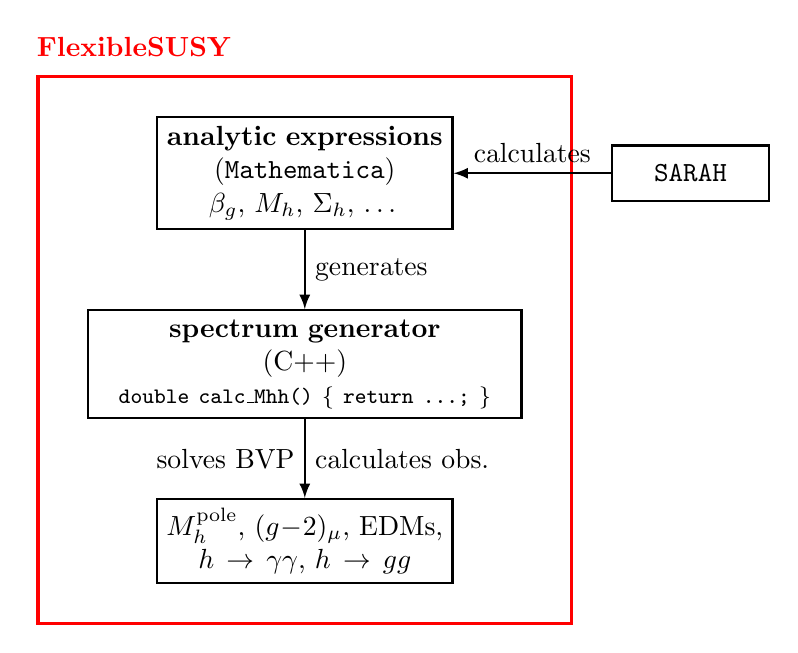
\begin{tikzpicture}
    \node[block] (EXPR) {\textbf{analytic expressions}\\ (\Mathematica)\\ $\beta_g$, $M_h$, $\Sigma_h$, \ldots};
    % \node[block, below = 1cm of EXPR, text width=15em] (FS) {\textbf{spectrum generator}\\ (C++)\\ solves BVP, calculates observables};
    \node[block, below = 1cm of EXPR, text width=15em] (FS) {\textbf{spectrum generator}\\ (C++)\\ \footnotesize{\texttt{double calc\_Mhh() \{ return ...; \}}}};
    \node[block, below = 1cm of FS] (OUT) {$M_h^\pole$, $(g-2)_\mu$, EDMs, $h\rightarrow\gamma\gamma$, $h\rightarrow gg$};
    \path[arrow] (EXPR) -- node[right]{generates} (FS);
    \path[arrow] (FS) -- node[right]{calculates obs.} node[left]{solves BVP} (OUT);
    \draw[red,very thick] ($(EXPR.north west)+(-1.5,0.5)$) node(FSname){} rectangle ($(OUT.south east)+(1.5,-0.5)$);
    \node[above right = 0cm and 0cm of FSname.north west] {\textbf{\textcolor{red}{FlexibleSUSY}}};
    \node[block, right = 2cm of EXPR, text width=5em] (SARAH) {\textbf{\SARAH}};
    \path[arrow] (SARAH) -- node[above]{calculates} (EXPR);
    \end{tikzpicture}
  \end{center}
\end{frame}

\begin{frame}{Example: BVP in the CMSSM}
  \begin{center}
  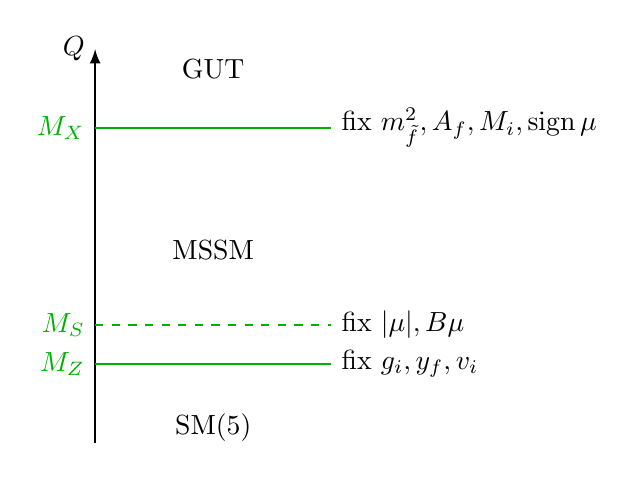
\begin{tikzpicture}
    \path[arrow] (0,0) -- (0,5) node[left]{$Q$};
    \draw[thick,darkgreen] (0,4) node[left]{$M_X$} -- node[above = 0.5cm,black]{GUT} (3,4) node[right,black]{fix $m_{\tilde{f}}^2, A_f, M_i, \sign\mu$};
    \draw[thick,dashed,darkgreen] (0,1.5) node[left]{$M_S$} -- (3,1.5) node[right,black]{fix $|\mu|, B\mu$};
    \draw[thick,darkgreen] (0,1) node[left]{$M_Z$} -- node[above = 1.2cm,black]{MSSM} node[below = 0.5cm,black]{SM(5)} (3,1) node[right,black]{fix $g_i, y_f, v_i$};
  \end{tikzpicture}
  \end{center}
\end{frame}

\begin{frame}{Example: BVP in the MSSM with light Higgs sector}
  \begin{center}
  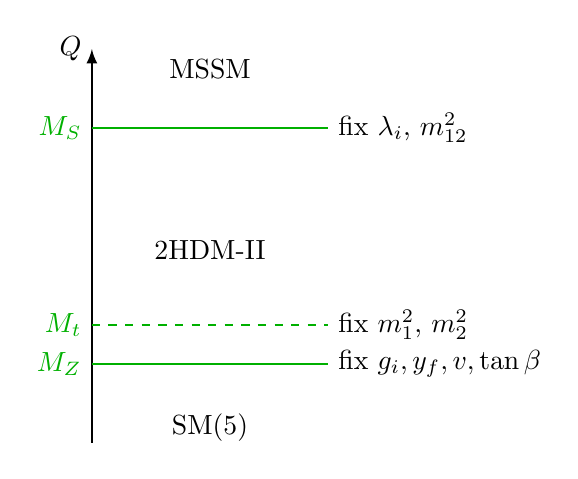
\begin{tikzpicture}
    \path[arrow] (0,0) -- (0,5) node[left]{$Q$};
    \draw[thick,darkgreen] (0,4) node[left]{$M_S$} -- node[above = 0.5cm,black]{MSSM} (3,4) node[right,black]{fix $\lambda_i$, $m_{12}^2$};
    \draw[thick,dashed,darkgreen] (0,1.5) node[left]{$M_t$} -- (3,1.5) node[right,black]{fix $m_1^2$, $m_2^2$};
    \draw[thick,darkgreen] (0,1) node[left]{$M_Z$} -- node[above = 1.2cm,black]{2HDM-II} node[below = 0.5cm,black]{SM(5)} (3,1) node[right,black]{fix $g_i, y_f, v, \tan\beta$};
  \end{tikzpicture}
  \end{center}
\end{frame}

\section{Features}

\newenvironment{obsblock}[1]{%
  \setbeamercolor{block body}{bg=darkgreen!10}
  \setbeamercolor{block title}{bg=darkgreen}
  \begin{block}{#1}}{\end{block}}

\newenvironment{precblock}[1]{%
  \setbeamercolor{block body}{bg=darkred!10}
  \setbeamercolor{block title}{bg=darkred}
  \begin{block}{#1}}{\end{block}}

\newenvironment{flexblock}[1]{%
  \setbeamercolor{block body}{bg=blue!10}
  \setbeamercolor{block title}{bg=blue}
  \begin{block}{#1}}{\end{block}}

\newenvironment{speedblock}[1]{%
  \setbeamercolor{block body}{bg=black!10}
  \setbeamercolor{block title}{bg=black}
  \begin{block}{#1}}{\end{block}}

\begin{frame}{Features for all models (SUSY and non-SUSY)}
  \begin{columns}[T]
    \begin{column}{0.49\textwidth}
      \begin{obsblock}{Observables}
        $M_h$, $M_W$, BSM masses, $(g-2)_\mu$, EDMs,
        $h\rightarrow\gamma\gamma$, $h\rightarrow gg$
      \end{obsblock}
      \begin{flexblock}{Flexibility}
        multipe BVP solvers, user-defined BCs, modular C++ code, SLHA
        input/output, \Mathematica\ input/output, SQLite output
      \end{flexblock}
    \end{column}
    \begin{column}{0.49\textwidth}
      \begin{precblock}{High precision}
        2L RGEs + 1L self energies (via \SARAH) + 1L thresholds,
        NNLL resummation for $M_h$ (\texttt{FlexibleEFTHiggs})
      \end{precblock}
      \begin{speedblock}{Speed}
        multi-threading, expression templates, lazy evaluation
      \end{speedblock}
    \end{column}
  \end{columns}
\end{frame}

\newenvironment{modelblock}[1]{%
  \setbeamercolor{block body}{bg=darkyellow!15}
  \setbeamercolor{block title}{fg=black,bg=darkyellow}
  \begin{block}{#1}}{\end{block}}

\begin{frame}{Additional model-specific precision corrections}
  \begin{columns}[T]
    \begin{column}{0.49\textwidth}
      \begin{modelblock}{MSSM}
        3L RGEs, 3L $M_h$, 2L $M_{H,A,H^\pm}$, 2L $(g-2)_\mu$, 2L
        thresholds
      \end{modelblock}
      \begin{modelblock}{NMSSM}
        2L $M_h$, 2L $M_{H,A,H^\pm}$, 2L thresholds
      \end{modelblock}
      \begin{modelblock}{Split-MSSM}
        3L $M_h$, 2L thresholds for $y_t$, 2L thresholds for $\lambda$, $\tilde{g}_{ip}$
        the MSSM
      \end{modelblock}
    \end{column}
    \begin{column}{0.49\textwidth}
      \begin{modelblock}{SM}
        3L RGEs, 3L $M_h$, 3L thresholds for $\as$, $y_{t,b}$, 2L
        thresholds for $\lambda$ to the MSSM (\texttt{HSSUSY})
      \end{modelblock}
      \begin{modelblock}{THDM-II}
        2L thresholds for $\lambda_i$ to the MSSM
      \end{modelblock}
      \begin{modelblock}{THDM-II + $\tilde{h}$ + $\tilde{g}$}
        1L thresholds for $\lambda_i$ to the MSSM
      \end{modelblock}
    \end{column}
  \end{columns}
\end{frame}

\section{Hands-on example: High-scale MSSM (HSSUSY)}

\begin{frame}{Hands-on example: High-scale MSSM (HSSUSY)}
  \begin{center}
  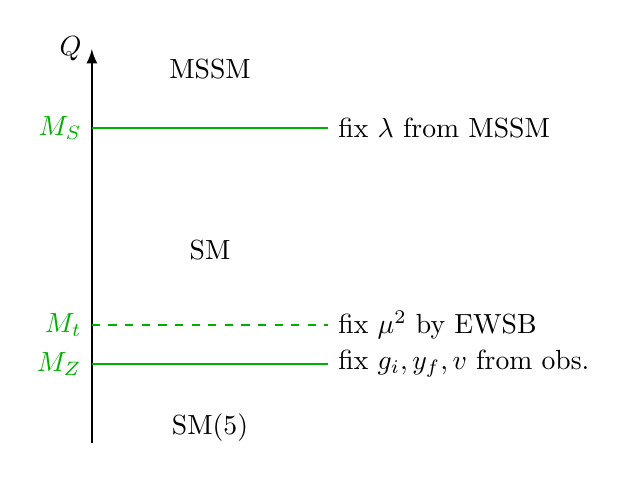
\begin{tikzpicture}
    \path[arrow] (0,0) -- (0,5) node[left]{$Q$};
    \draw[thick,darkgreen] (0,4) node[left]{$M_S$} -- node[above = 0.5cm,black]{MSSM} (3,4) node[right,black]{fix $\lambda$ from MSSM};
    \draw[thick,dashed,darkgreen] (0,1.5) node[left]{$M_t$} -- (3,1.5) node[right,black]{fix $\mu^2$ by EWSB};
    \draw[thick,darkgreen] (0,1) node[left]{$M_Z$} -- node[above = 1.2cm,black]{SM} node[below = 0.5cm,black]{SM(5)} (3,1) node[right,black]{fix $g_i, y_f, v$ from obs.};
  \end{tikzpicture}
  \end{center}
\end{frame}

\newsavebox{\listbox}

\begin{lrbox}{\listbox}\begin{lstlisting}[language=Mathematica]
LagNoHC = mu2 conj[H].H -
          1/2 \[Lambda] conj[H].H.conj[H].H;
LagHC   = -(Yd conj[H].d.q + Ye conj[H].e.l
            + Yu u.q.H);
\end{lstlisting}\end{lrbox}

\begin{frame}{Step 0: Chose a \SARAH\ model}
  We chose \SARAH's \texttt{SM} model with the parameters:
  \begin{center}
  \lstinline{g1}, \lstinline{g2}, \lstinline{g3}, \lstinline{Yu},
  \lstinline{Yd}, \lstinline{Ye}, \lstinline{\\[Lambda]},
  \lstinline{mu2}, \lstinline{v}
  \end{center}
  and the non-interaction Lagrangian \\[2em]
  \usebox{\listbox}
\end{frame}

\begin{lrbox}{\listbox}\begin{lstlisting}[language=bash]
$ cd FlexibleSUSY/
$ mkdir model_files/HSSUSY/
$ touch model_files/HSSUSY/FlexibleSUSY.m.in
\end{lstlisting}\end{lrbox} % $

\begin{frame}{Step 1: Create FlexibleSUSY model file}
  \usebox{\listbox}
\end{frame}

\begin{lrbox}{\listbox}\begin{lstlisting}[language=Mathematica]
FSModelName = "HSSUSY";
FSEigenstates = SARAH`EWSB;
FSDefaultSARAHModel = SM;
\end{lstlisting}\end{lrbox}

\begin{frame}{Step 2: Define model information}
  Put into the model file
  \lstinline{model_files/HSSUSY/FlexibleSUSY.m.in}:
  \\[2em]
  \usebox{\listbox}
\end{frame}

\begin{lrbox}{\listbox}\begin{lstlisting}[language=Mathematica]
EXTPAR = {
    {0, MS},
    {1, M1Input},
    {2, M2Input},
    {3, M3Input},
    {4, MuInput},
    {5, mAInput},
    {6, MEWSB},
    {7, AtInput},
    {25, TanBeta}
};

FSAuxiliaryParameterInfo = {
    {msq2, { LesHouches -> MSQ2IN,
             ParameterDimensions -> {3,3},
             InputParameter -> True } },
    ...
};
\end{lstlisting}\end{lrbox}

\begin{frame}{Step 3: Define MSSM input parameters}
  \usebox{\listbox}
\end{frame}

\begin{lrbox}{\listbox}\begin{lstlisting}[language=Mathematica]
LowScale = LowEnergyConstant[MZ];

LowScaleInput = {
   {v, 2 MZMSbar / Sqrt[3/5 g1^2 + g2^2]},
   {Yu, Automatic},
   {Yd, Automatic},
   {Ye, Automatic}
   (* gauge couplings are fixed automatically *)
};
\end{lstlisting}\end{lrbox}

\begin{frame}{Step 4: Define low-scale boundary condition}
  Fix $v^{\MSbar}$, $y_f^{\MSbar}$ and $g_i^{\MSbar}$ at the scale $Q = M_Z$:\\[2em]
  \usebox{\listbox}
  \\[1em]
  \lstinline{MZMSbar} = $m_Z^{\MSbar}(Q)$
\end{frame}

\begin{lrbox}{\listbox}\begin{lstlisting}[language=Mathematica]
EWSBOutputParameters = { mu2 };

SUSYScale = MEWSB;

SUSYScaleInput = {
   FSSolveEWSBFor[EWSBOutputParameters]
};
\end{lstlisting}\end{lrbox}

\begin{frame}{Step 5: Define EWSB-scale boundary condition}
  Fix $\mu^2$ by EWSB condition at the scale $Q$ = \lstinline{MEWSB}:\\[2em]
  \usebox{\listbox}
\end{frame}

\begin{lrbox}{\listbox}\begin{lstlisting}[language=Mathematica]
HighScale = MS;

HighScaleInput = {
    {\[Lambda],
       (3/5 g1^2 + g2^2)/4 Cos[2 ArcTan[TanBeta]]^2
    }
};
\end{lstlisting}\end{lrbox}

\begin{frame}{Step 6: Define high-scale boundary condition}
  Fix $\lambda$ by matching to the MSSM the scale $Q$ = \lstinline{MS}:
  \begin{align*}
    \lambda(Q) = \frac{1}{4} \left[ \frac{3}{5} g_1^2(Q) + g_2^2(Q) \right] \cos^2 {2\beta}
    \qquad \text{\mycite{0705.1496}}
  \end{align*}
  \\[1em]
  \usebox{\listbox}
\end{frame}

\begin{lrbox}{\listbox}\begin{lstlisting}[language=Mathematica]
UseSM3LoopRGEs    = True; (* 3L RGEs *)
UseYukawa3LoopQCD = True; (* 3L corr. to yt *)
UseSMAlphaS3Loop  = True; (* 3L corr. to alpha_s *)
UseHiggs2LoopSM   = True; (* 2L contributions to Mh *)
UseHiggs3LoopSM   = True; (* 3L contributions to Mh *)
\end{lstlisting}\end{lrbox}

\begin{frame}{Step 7: Enable SM-specific higher order corrections}
  Higher-order corrections from the literature \mycite{hep-ph/9911434,
    hep-ph/9912391, hep-ph/0004189, 1407.4336}:
  \begin{align*}
    m_t &= M_t + \Delta^{(1)} m_t + \Delta^{(2)} m_t + \Delta^{(3)} m_t \\
    \alpha_s &= \frac{\alpha_s^{\SM(5)}}{1 + \Delta^{(1)} \as + \Delta^{(2)} \as + \Delta^{(3)} \as} \\
    M_h^2 &= m_h^2 + \Delta^{(1)} m_h^2 + \Delta^{(2)} m_h^2 + \Delta^{(3)} m_h^2
  \end{align*}
  \\[1em]
  \usebox{\listbox}
\end{frame}

\begin{lrbox}{\listbox}\begin{lstlisting}[language=bash]
$ ./createmodel --name=HSSUSY
$ ./configure --with-models=HSSUSY
$ make -j4
\end{lstlisting}\end{lrbox} % $

\begin{frame}{Finally: Build the spectrum generator}
  \usebox{\listbox}
  \\[1em]
  \begin{itemize}
  \item[\texttt{1}:] creates the directory \lstinline{models/HSSUSY/}
    with makefile module
  \item[\texttt{2}:] checks the system and creates the \lstinline{Makefile}
  \item[\texttt{3}:] generates the C++ code and compiles it
  \end{itemize}
\end{frame}

\begin{lrbox}{\listbox}\begin{lstlisting}[language=bash]
$ cd models/HSSUSY/
$ ./run_HSSUSY.x \
    --slha-input-file=LesHouches.in.HSSUSY
Block SPINFO
     1   FlexibleSUSY
     2   2.0.1
     5   HSSUSY
     9   4.12.0
Block MASS
        24     8.03785042E+01   # VWp
        25     1.14703451E+02   # hh
...
\end{lstlisting}\end{lrbox} % $

\begin{frame}{Run HSSUSY}
  Run HSSUSY using an SLHA input file:\\[2em]
  \usebox{\listbox}
\end{frame}

\begin{lrbox}{\listbox}\begin{lstlisting}[language=Mathematica]
Get["models/HSSUSY/HSSUSY_librarylink.m"];
\end{lstlisting}\end{lrbox} % $

\begin{frame}{Let's make a plot!}
  We'll use the \Mathematica\ interface of FlexibleSUSY to perform a
  scan over $\MS$.\\[1em]
  Open \Mathematica\ and type:\\[2em]
  \usebox{\listbox}
  \\[1em]
  Now we can use these functions (and more):\\
  \begin{itemize}
  \item[] \texttt{FSHSSUSYOpenHandle[<parameters>]}
  \item[] \texttt{FSHSSUSYCloseHandle[<handle>]}
  \item[] \texttt{FSHSSUSYCalculateSpectrum[<handle>]}
  \item[] \ldots
  \end{itemize}
\end{frame}

\begin{lrbox}{\listbox}\begin{lstlisting}[language=Mathematica]
handle = FSHSSUSYOpenHandle[
    fsSettings -> {
        calculateStandardModelMasses -> 1
    },
    fsModelParameters -> {
        TanBeta -> 5,
        MEWSB -> 173.34,
        MSUSY -> 5000,
        M1Input -> 5000,
        M2Input -> 5000,
        M3Input -> 5000,
        MuInput -> 5000,
        mAInput -> 5000,
        AtInput -> 1000,
        msq2 -> 5000^2 IdentityMatrix[3],
        msu2 -> 5000^2 IdentityMatrix[3],
        msd2 -> 5000^2 IdentityMatrix[3],
        msl2 -> 5000^2 IdentityMatrix[3],
        mse2 -> 5000^2 IdentityMatrix[3]
    }
];

spec = FSHSSUSYCalculateSpectrum[handle];

FSHSSUSYCloseHandle[handle];
\end{lstlisting}\end{lrbox} % $

\begin{frame}{Let's make a plot!}
  \usebox{\listbox}
\end{frame}

\begin{lrbox}{\listbox}\begin{lstlisting}[language=Mathematica]
In[]:= Print[spec];

Out[]=
{HSSUSY -> {
   M[hh] -> 116.74076603621857,
   M[VWp] -> 80.16049791392693,
   Pole[M[hh]] -> 117.38153372733366,
   Pole[M[VWp]] -> 80.37359140369604,
   ...
   \[Lambda] -> 0.22248507579380888,
   Yu -> {{7.493388340878909*^-6, 0., 0.},
          {0., 0.003411223511630361, 0.},
          {0., 0., 0.9384438041061343}},
   ...
   SCALE -> 173.34
 }
}
\end{lstlisting}\end{lrbox} % $

\begin{frame}{Let's make a plot!}
  \usebox{\listbox}
\end{frame}

\begin{lrbox}{\listbox}\begin{lstlisting}[language=Mathematica]
CalcMh[MS_, TB_, Xtt_] :=
    Module[{handle, spec},
        handle = FSHSSUSYOpenHandle[
            fsSettings -> { ... },
            fsSMParameters -> { ... },
            fsModelParameters -> {
                TanBeta -> TB, MEWSB -> 173.34, MSUSY -> MS,
                M1Input -> MS, M2Input -> MS, M3Input -> MS,
                MuInput -> MS, mAInput -> MS,
                AtInput -> (Xtt + 1/TB) MS,
                msq2 -> MS^2 IdentityMatrix[3],
                msu2 -> MS^2 IdentityMatrix[3],
                msd2 -> MS^2 IdentityMatrix[3],
                msl2 -> MS^2 IdentityMatrix[3],
                mse2 -> MS^2 IdentityMatrix[3]
            }
        ];
        spec = FSHSSUSYCalculateSpectrum[handle];
        FSHSSUSYCloseHandle[handle];
        Pole[M[hh]] /. (HSSUSY /. spec)
       ];
\end{lstlisting}\end{lrbox} % $

\begin{frame}{Let's make a plot!}
  Wrap everything into a function:\\[1em]
  \usebox{\listbox}
\end{frame}

\begin{lrbox}{\listbox}\begin{lstlisting}[language=Mathematica]
LogRange[start_, stop_, steps_] :=
    Exp /@ Range[Log[start], Log[stop],
                 (Log[stop] - Log[start])/steps];

LaunchKernels[];
DistributeDefinitions[CalcMh];

data = ParallelMap[{ N[#], CalcMh[#, 5, 0] }&,
                   LogRange[300, 5 10^4, 100]
       ];
\end{lstlisting}\end{lrbox} % $

\begin{frame}{Let's make a plot!}
  Scan over $\MS \in [0.3, 5]\eh{TeV}$ with $X_t = 0$, $\tan\beta = 5$:\\[2em]
  \usebox{\listbox}
\end{frame}

\begin{frame}{Let's make a plot!}
  \begin{center}
    \includegraphics[width=0.6\textwidth]{plots/HSSUSY/Mh_MS_TB-5_Xt-0}
  \end{center}
\end{frame}

\begin{lrbox}{\listbox}\begin{lstlisting}[language=bash]
HighScaleInput = {
   {\[Lambda], lambdaTree + lambda1L}
};

lambdaTree = (3/5 g1^2 + g2^2)/4 Cos[2 ArcTan[TanBeta]]^2;

lambda1L = With[{yt = Yu[3,3],
                 Xt = AtInput - MuInput/TanBeta},
   3/8 yt^4/Pi^2 ( Xt^2/MS^2 - Xt^4/(12 MS^4) )
];
\end{lstlisting}\end{lrbox} % $

\begin{frame}{Let's add 1-loop corrections for $\lambda$}
  Let's implement the leading 1-loop correction from
  \bigcite{0705.1496}:
  \begin{align*}
    \lambda(Q) &= \frac{1}{4} \left[ \frac{3}{5} g_1^2 + g_2^2 \right] \cos^2 2\beta
    + \frac{3}{8} \frac{y_t^4}{\pi^2}\left[
       \frac{X_t^2}{\MS^2}
       - \frac{X_t^4}{12 \MS^4}
    \right]
  \end{align*}
  with $X_t = A_t - \mu/\tan\beta$.
  In the HSSUSY model file this reads:\\[2em]
  \usebox{\listbox}
\end{frame}

\begin{lrbox}{\listbox}\begin{lstlisting}[language=Mathematica]
MS = 5000;
TB = 5;

data = ParallelMap[{ N[#], CalcMh[MS, TB, #] }&,
                   Range[-3.5, 3.5, 0.1]
       ];
\end{lstlisting}\end{lrbox} % $

\begin{frame}{Let's make a plot!}
  Scan over $X_t/\MS \in [-3.5, 3.5]$ with $\MS = 5\eh{TeV}$, $\tan\beta = 5$:\\[2em]
  \usebox{\listbox}
\end{frame}

\begin{frame}{Tree-level vs.\ leading 1-loop vs.\ leading 2-loop}
  \begin{center}
    \includegraphics[width=0.6\textwidth]{plots/HSSUSY/Mh_Xt_TB-5_MS-5000}
  \end{center}
  2-loop contributions from \bigcite{1407.4081, 1703.08166}.
\end{frame}

\begin{lrbox}{\listbox}\begin{lstlisting}[language=bash]
EXTPAR = {
   ...
   {DeltaEFT, 100}
};

HighScaleInput = {
   {\[Lambda], lambdaTree + lambda1L + lambda1LEFT}
};

lambdaTree  = ...;
lambda1L    = ...;
lambda1LEFT = DeltaEFT Yu[3,3]^4/(4 Pi)^2 v^2/MS^2;
\end{lstlisting}\end{lrbox} % $

\begin{frame}{Estimate the EFT uncertainty}
  The pure EFT calculation neglects terms of $O(v^2/\MS^2)$.\\
  Estimate these terms by adding
  \begin{align*}
    \lambda(Q) &= \lambda^{(0L)} + \Delta\lambda^{(1L)}
    + \delta_\text{EFT} \frac{y_t^4}{(4\pi)^2} \frac{v^2}{\MS^2}
  \end{align*}
  with $\delta_\text{EFT} = 0$ or $1$.\\[1em]
  \usebox{\listbox}
\end{frame}

\begin{lrbox}{\listbox}\begin{lstlisting}[language=Mathematica]
CalcMh[MS_, TB_, Xtt_, deltaEFT_] :=
    Module[{handle, spec},
        handle = FSHSSUSYOpenHandle[
            fsSettings -> { ... },
            fsSMParameters -> { ... },
            fsModelParameters -> {
                ...
                DeltaEFT -> deltaEFT (* <-- set DeltaEFT *)
            }
        ];
        spec = FSHSSUSYCalculateSpectrum[handle];
        FSHSSUSYCloseHandle[handle];
        Pole[M[hh]] /. (HSSUSY /. spec)
       ];
\end{lstlisting}\end{lrbox} % $

\begin{frame}{Let's make a plot!}
  Extend our wrapper function:\\[2em]
  \usebox{\listbox}
\end{frame}

\begin{lrbox}{\listbox}\begin{lstlisting}[language=Mathematica]
data = ParallelMap[{ N[#],
                     CalcMh[#, 5, 0, 0],
                     CalcMh[#, 5, 0, 1] }&,
                   LogRange[100, 5 10^4, 100]
       ];
\end{lstlisting}\end{lrbox} % $

\begin{frame}{Let's make a plot!}
  Scan over $\MS \in [0.1, 5]\eh{TeV}$ with $X_t = 0$, $\tan\beta = 5$:\\[2em]
  \usebox{\listbox}
\end{frame}

\begin{frame}
  \includegraphics[width=0.49\textwidth]{plots/HSSUSY/Mh_MS_TB-5_Xt-0_EFT}\hfill
  \includegraphics[width=0.49\textwidth]{plots/HSSUSY/Mh_MS_TB-5_Xt-0_EFT_uncertainty}
\end{frame}

\end{document}
